% chktex-file -1
% chktex-file 24
% chktex-file 9
\chapter{Method}
\label{cha:method}

This chapter describes the theory used and developed in this thesis. The
notation for HMMs introduced in section~\ref{sec:hidden-markov-models} is
written out as this is used extensively in the following sections.

The first contribution of this thesis is the reformulation of the original
Viterbi algorithm to fit into the zipHMM framework, to analyze the running
time, and to make the computations numerically stable.

Next, theory for the posterior decoding is described. As only the forward
algorithm has been implemented in zipHMM the backward algorithm is described
here since it is required to compute the posterior decoding. However, it is has
not been possible to develop an algorithm for exploiting repetitions.

The final theoretical contribution is the theory for an \emph{indexed}
posterior decoding. A theoretical speedup can be gained by exploiting
repetitions in the entire input sequence for the forward and backward
algorithms and only return the posterior decoding for a part of the input
sequence.

\section{Notation}

Recall the introduction to HMM's given in
section~\ref{sec:hidden-markov-models}. An HMM can generate an \emph{observation
 sequence} $Y_{1:T} = y_1y_2\dots{}y_T$ with $y_i \in \mathcal{O}$ by
traversing hidden states and emitting symbols. There exist one or more
\emph{paths} of hidden states $V_{1:T} = v_1v_2\dots{}v_T$ with
$v_i \in \mathcal{H}$ for each observation sequence generated by the HMM.\@ Formally
a HMM is defined as
\begin{itemize}
\item $\mathcal{H} = \{h_1, h_2, \dots, h_N\}$, a finite alphabet of hidden
  states;
\item $\mathcal{O} = \{o_1, o_2, \dots, o_M\}$, a finite alphabet of observables;
\item a vector $\Pi = {\{\pi_i\}}_{1 \le i \le N}$, where $\pi_i = \Pr(v_1 =
  h_i)$ is the probability of the model starting in hidden state $h_i$;
\item a matrix $A = {\{a_{ij}\}}_{1 \le i \le N}$, where $a_{ij} = \Pr(v_t
  = h_j \mid v_{t - 1} = h_i)$ is the probability of a transition from state
  $h_i$ to state $h_j$;
\item a matrix $B = {\{b_{ij}\}}_{1 \le i \le N}^{1 \le j \le M}$, where
  $b_{ij} = \Pr(y_t = o_j \mid v_t = h_i)$ is the probability of state
  $h_i$ emitting $o_j$.
\end{itemize}
A HMM is parametrized by $\pi$, $A$, and $B$ and is denoted by $\lambda =
(\pi, A, B)$.

\section{The Original Viterbi Algorithm}
\label{sec:class-viterbi-algor}

As mentioned in section~\ref{sec:hidden-markov-models} an observation sequence
$Y_{1:T}$ can be generated in different ways since multiple hidden states can
have a nonzero probability of omitting the same symbol. Given a model $\lambda$
and an observation sequence an interesting question might be: of all possible
paths of hidden sequences which one is the most likely and how likely is it?
This question can be solved the Viterbi algorithm.

The Viterbi algorithm finds the probability of the most likely sequence of
hidden states emitting an observation sequence $Y_{1:T}$ given a model
$\lambda$. This can be expressed as maximizing the probability of the
observation and hidden sequences for all possible hidden sequences, that is
$\max_{v_{1:T}} \Pr(Y_{1:T}, V_{1:T} = v_{1:T} \mid \lambda)$.

To compute this, consider the Viterbi variable $\delta_t(v_t)$ defined as
\begin{equation*}
  \delta_t(v_t) = \max_{v_{1:t}} \Pr(Y_{1:t}, V_{1:t} = v_{1:t} \mid \lambda).
\end{equation*}
This is the probability of the partial observation sequence $Y_{1:t}$ at time
$t$ plus the probability of the most likely sequence of states $V_{1:t}$. Since
the probability of making a transition to the next state is only dependent on
the current state, this formula is solved inductively by
\begin{equation}
  \label{eq:1}
  \begin{aligned}
    \delta_1(v_1) &= \pi_{v_1} b_{v_1, y_1} \\
    \delta_t(v_t) &= b_{v_t, y_t} \max_{v_{t - 1}} \delta_{t - 1}(v_{t - 1}) a_{v_{t - 1}, v_t}.
  \end{aligned}
\end{equation}
This is computed efficiently by making $\delta$ a table of size
$N \times T$ and by computing this table column-wise from left to right
using dynamic programming. After populating $\delta$,
the probability of the most likely sequence of states can be computed as
$P^* = \max_{v_T} \delta_T(v_T)$.

The most likely sequence of hidden states $V_{1:T}^* = v_1^*v_2^*\dots{}v_T^*$,
also known as the \emph{Viterbi path}, can be computed similarly. Another table
$\Psi$ of the same size as $\delta$ is computed along $\delta$ with pointers
from each state in a column to the maximizing previous state:
\begin{equation*}
  \begin{aligned}
    \Psi_1(v_1) &= 0 \\
    \Psi_t(v_t) &= \argmax_{v_{t - 1}} \delta_{t - 1}(v_{t - 1}) a_{v_{t - 1}, v_t}.
  \end{aligned}
\end{equation*}
When the last column has been computed in $\delta$ and $\Psi$ the last state
in the Viterbi path is found using
\begin{equation*}
  v_T^* = \argmax_{v_T} \delta_T(v_T).
\end{equation*}
From this state the entire Viterbi path $V_T^*$ can be found by backtracking
the pointers in the table using
\begin{equation*}
  v_t^* = \Psi_{t + 1}(v_{t + 1}^*).
\end{equation*}

\subsection{Running Time}

Note that if only the probability is needed, only the last filled out column of
$\delta$ needs to be stored since the recursion in equation~\eqref{eq:1} only
needs the previous column to compute the new one. Hence, the space consumption
of the algorithm will be the space needed for two columns and the observation
sequence, that is $O(N + T)$. To compute a cell in $\delta$ the algorithm
maximizes over all cells in the previous column resulting in a running time of
$O(N^2 T)$.

The space consumption of this backtracking algorithm is the size of $\Psi$
which is $O(N T)$. Backtracking is computed in $O(T)$ time, since it is only
lookups in $\Psi$.

A space consumption of $O(N T)$ might be too large for some applications;
especially the $T$ factor can become large. Another way to backtrack is
described by \citet{Tarnas01061998}. By using this approach the space
consumption is reduced to $O(N \sqrt{T})$ while the asymptotic running
time of the algorithm is preserved.

The $\delta$ table is split into blocks of size $B$. While computing $\delta$,
the first column of each block in stored, while the rest is thrown away. These
columns is called checkpoints. Since computing a column only requires the
previous column as seen in equation~(\ref{eq:1}), the part of the
$\delta$ table corresponding to a block can be computed using the checkpoint,
and thereby $\Psi$ can also be computed. When the last column in $\delta$ has
been computed, $v_T^*$ can be found as described above. The blocks are then
recomputed one at a time from right to left. When the $\Psi$ table for a block
has been recomputed it is backtracked as before. Hence, only one block is kept
in memory at a time. If $B = \sqrt{T}$ is chosen, the space consumption is
$O(N T / B) = O(N T / \sqrt{T}) = O(N \sqrt{T})$. $\delta$ is now computed two times, so
the algorithm is slower, but the algorithm keeps having the same
asymptotic running time of $O(N^2 T)$.

\section{Viterbi as Linear Algebra}
\label{sec:algorithm-as-linear}

Before exploiting repetitions in the observation sequence $Y_{1:T}$ the
original Viterbi algorithm is reformulated into linear algebra. The goal is to
express equation~\eqref{eq:1} as a series of matrix multiplications as
\citet{sand2013ziphmmlib} and \citet{lifshits2009speeding} do.

For each symbol $o_i \in \mathcal{O}$, let $B_{o_i}$ be the diagonal matrix
having the emission probabilities of $o_i$ of the diagonal:
\begin{equation*}
  B_{o_i} =
  \begin{bmatrix}
    b_{1, o_i} &            &        &            \\
               & b_{2, o_i} &        &            \\
               &            & \cdots &            \\
               &            &        & b_{N, o_i} \\
  \end{bmatrix}
\end{equation*}
and let
\begin{align*}
  C_{o_i}      & = B_{o_i} A^T                    \\
  C_1          & = B_{y_1} \pi,
\end{align*}
where $A^T$ is the transpose of $A$. Each matrix $C_{o_i}$ is of size $N \times
N$ and an entry $C_{o_i}(k, l)$ is probability of making a transition
from state $k$ to state $l$ and emit symbol $o_i$.

Equation~\eqref{eq:1} can now be expressed by these matrices. It is trivial to
see that the base case is $C_1$. For the recursive case we note that
$x \max_k y z = \max_k x y z$. Hence, $\delta_t$ can be computed using $C_{y_t}$
and $\delta_{t - 1}$ using the recursive formula
\begin{equation}
  \label{eq:2}
  \begin{aligned}
    \delta_1 &= C_1 \\
    \delta_t &= C_{y_t} \odot \delta_{t - 1} = C_{y_t} \odot C_{y_{t-1}} \odot \dots \odot C_1,
  \end{aligned}
\end{equation}
where $\odot$ is the max-times matrix multiplication defined as
\begin{equation*}
{(X \odot Y)}_{ij} = \max_k X_{ik} Y_{kj}.
\end{equation*}

The implementation of the original Viterbi algorithm corresponds to
computing this from right to left, i.e.\ the $\delta$ table is computed for $t
= 1, t=2, \dots, t=T$. This will also be most efficient since
$C_1$ is a vector that when multiplied by the matrix $C_2$ will result in a new
vector. Hence, computing $\delta_t$ from right to left will result in $t$
matrix-vector multiplications, while computing it from left to right will
result in $t$ matrix-matrix multiplications that are less efficient to compute.

Backtracking is achieved in the same way as for the original Viterbi algorithm
as described in section~\ref{sec:class-viterbi-algor}.

The space consumption and running time of this algorithm has changed, compared
to the original Viterbi algorithm. For each symbol $o_i$ in the alphabet of
observables the corresponding matrix $B_{o_i}$ is created, thus requiring
$O(M N^2)$ space. The $C_{o_i}$ matrices require the same amount of space,
$O(M N^2)$. $C_1$ is a vector, thus only requiring $O(N)$ space. If
equation~\eqref{eq:2} is evaluated from right to left it corresponds to a
series of matrix-vector multiplications resulting in a vector of size $O(N)$.
In total this requires $O(2 M N^2 + 2 N) = O(M N^2)$ space. If backtracking is
required, the space consumption will be increased by the size of the $\Psi$
table that has size $O(N T)$. The total the space consumption with backtracking
enabled is $O(M N^2 + N T)$, or if the checkpoint trick is used, $O(M N^2 +
N \sqrt{T})$.

Likewise, the running time has changed. Creating the $B_{o_i}$ matrices takes
$O(M N^2)$ time. Computing the $C_{o_i}$ matrices takes time $O(M N^3)$ due to
the matrix multiplication. Computing $C_1$ takes $O(N^2)$ times. Again, if
equation~\eqref{eq:2} is evaluated from right to left, it will be matrix-vector
multiplications requiring $O(N^2 T)$ time. Backtracking can be computed in either
$O(NT)$ or $O(N^2 T)$ time by using the $\Psi$ table. In total this becomes
$O(M N^2 + M N^3 + N^2 + N^2 T) = O(M N^3 + N^2 T)$.

\section{Exploiting Repetitions}
\label{sec:expl-repet}

In this section it is shown how to exploit repetitions in the observation sequence
to make the above algorithm run faster. \citet{lifshits2009speeding} introduces
five different methods for compression, while \citet{sand2013ziphmmlib} only uses
byte-pair encoding.

\subsection{Byte-Pair Encoding}

Byte-pair encoding is a simple data compression method. The most common pair
consecutive bytes in the data is replaced by a byte that does not exist in the
data. This is repeated until either all new bytes are used or the most common
pair does not appear frequently in the data. The use of bytes can easily be
replaced by used of characters or integers. For example, the input sequence
01012012 would first be encoded into 33232 by substituting 01 with 3; in the
next iteration it would be encoded into 344 by substituting 32 by 4 etc.

\subsection{Using Byte-Pair Encoding to Speed Up Viterbi}
\label{sec:using-byte-pair}

The Viterbi algorithm achieves a speed up using byte-pair encoding in the
following way. A the beginning of an iteration let $o_i o_j \in O \times O$ be
the most frequently occurring pair of symbols in $Y_{1:T}$ and let
$n_{o_i o_j}$ be the number of occurrences. $o_i o_j$ is substituted by a new
symbol $o_{M + 1}$ and the length of $Y_{1:T}$ is thereby reduced by
$n_{o_i o_j}$. All $n_{o_i o_j}$ occurrences of $C_{o_i} \odot C_{o_j}$ in
equation~\eqref{eq:2} can be replaced by the new matrix
\begin{equation}
  \label{eq:7}
  C_{o_{M + 1}} = C_{o_i} \odot C_{o_j}.
\end{equation}
Hence, the number of matrix multiplications is reduced by $n_{o_i o_j}$. The
byte-pair encoding continues with more iterations until $n_{o_i o_j}$ becomes
too small to give a speed up. This is discussed later. The result of this is a
new sequence $Y_{1:T'}'$ over the new alphabet
\begin{equation*}
  \begin{aligned}
    \mathcal{O}' & = \{o_1, o_2, \dots, o_M, o_{M + 1}, o_{M + 2}, \dots, o_{M'} \} \\
                 & = \{o_1, o_2, \dots, o_M, (l_1, r_1), (l_2, r_2), \dots, (l_{M' - M}, r_{M' - M}) \},
  \end{aligned}
\end{equation*}
where $l_i, r_i \in \{o_1, o_2, \dots, o_{M + i - 1} \}$.

This method is split up into two separate computations. First the sequence
is encoded as just discussed. As the encoding of the sequence is independent of
the HMM the encoded sequence can be saved to disk for later use and can be
called preprocessing. The second part consist of the actual Viterbi algorithm
and is split into two stages. The first stage is the computation of
$C_{o_i}$ for $i = 1, \dots, M$ and then $C_{o_i}$ for increasing
$i = M + 1, \dots, M'$ by $C_{o_i} = C_{l_i} \odot C_{l_r}$. In the second
stage $\delta_T$ is computed by
\begin{equation}
  \label{eq:3}
  \delta_T = C_{y'_{T'}} \odot C_{y'_{T'-1}} \odot \dots \odot C_{y'_2} \odot C_1.
\end{equation}

An illustration of this method is given in
figure~\ref{fig:exploiting-repetitions}. As seen, when the computation has
finished only a subset of the columns of $\delta$ has been computed. As an
example consider the observation sequence $Y_{1:10} = 1010001001$ over the
alphabet $\mathcal{O} = \{0, 1\}$. This is being compressed by first replacing
the pair $10$ by a new symbol $2$, and the replacing $20$ by $3$. Hence, the
original observation sequence of length 10, becomes compressed to a sequence
$Y_{1:5}'$ of length 5. Now, for each symbol in the new alphabet
$\mathcal{O'} = \{0, 1, 2, 3\}$ the $C_{o_i}$ matrices and the $C_1$ matrix are
constructed. These corresponds to the rectangles with a thick line. The solid
lines correspond to the matrix multiplications performed, while the dotted
lines is the work saved due to redundancy. Finally, columns of $\delta$ is
computed by performing matrix-vector multiplications from right to left, while
the gray columns correspond to the amount of work saved in the Viterbi
computation.

\begin{figure}
  \centering
  \tikzsetnextfilename{exploiting_repetitions}
\begin{tikzpicture}[
  font=\scriptsize,
  ]
  \tikzstyle{matrix} = [minimum width=7mm, minimum height=7mm];
  \tikzstyle{vector} = [minimum width=3mm, inner sep=0mm, minimum height=7mm];

  \tikzstyle{symbol} = [matrix, draw=black];
  \tikzstyle{delta}  = [vector, draw=gray, text=gray];
  \tikzstyle{delta'} = [delta, draw=black, text=black];

  \tikzstyle{arrow} = [->]

  \node[symbol] (y10) at (0, 3) {1};
  \node[symbol] (y9) at (1, 3) {0};
  \node[symbol] (y8) at (2, 3) {0};
  \node[symbol] (y7) at (3, 3) {1};
  \node[symbol] (y6) at (4, 3) {0};
  \node[symbol] (y5) at (5, 3) {0};
  \node[symbol] (y4) at (6, 3) {0};
  \node[symbol, thick] (y3) at (7, 3) {1};
  \node[symbol, thick] (y2) at (8, 3) {0};
  \node[symbol, vector, thick] (y1) at (9, 3) {1};

  \node[symbol] (y+7) at (0, 2) {2};
  \node[symbol] (y+6) at (2, 2) {0};
  \node[symbol] (y+5) at (3, 2) {2};
  \node[symbol] (y+4) at (5, 2) {0};
  \node[symbol] (y+3) at (6, 2) {0};
  \node[symbol, thick] (y+2) at (7, 2) {2};
  \node[symbol, vector] (y+1) at (9, 2) {1};

  \node[symbol] (y'5) at (0, 1) {3};
  \node[symbol, thick] (y'4) at (3, 1) {3};
  \node[symbol] (y'3) at (6, 1) {0};
  \node[symbol] (y'2) at (7, 1) {2};
  \node[symbol, vector] (y'1) at (9, 1) {1};

  \node[left of=y10] {$Y_{1:10}$};
  \node[left of=y'5] {$Y_{1:5}'$};

  \path (y10) edge[arrow, dotted] (y+7);
  \path (y9) edge[arrow, dotted] (y+7);

  \path (y7) edge[arrow, dotted] (y+5);
  \path (y6) edge[arrow, dotted] (y+5);

  \path (y3) edge[arrow] (y+2);
  \path (y2) edge[arrow] (y+2);

  \path (y+7) edge[arrow,dotted] (y'5);
  \path (y+6) edge[arrow,dotted] (y'5);

  \path (y+5) edge[arrow] (y'4);
  \path (y+4) edge[arrow] (y'4);

  \node[delta'] (d10) at (0, -0.9) {$\delta_{10}$};
  \node[delta]  (d9)  at (1, -0.8) {$\delta_9$};
  \node[delta]  (d8)  at (2, -0.7) {$\delta_8$};
  \node[delta'] (d7)  at (3, -0.6) {$\delta_7$};
  \node[delta]  (d6)  at (4, -0.5) {$\delta_6$};
  \node[delta]  (d5)  at (5, -0.4) {$\delta_5$};
  \node[delta'] (d4)  at (6, -0.3) {$\delta_4$};
  \node[delta'] (d3)  at (7, -0.2) {$\delta_3$};
  \node[delta]  (d2)  at (8, -0.1) {$\delta_2$};
  \node[delta'] (d1)  at (9, 0) {$\delta_1$};

  \path (y'5) edge[arrow] (d10);
  \path (y'4) edge[arrow] (d7);
  \path (y'3) edge[arrow] (d4);
  \path (y'2) edge[arrow] (d3);
  \path (y'1) edge[arrow] (d1);

  \path (d1) edge[arrow] (d3);
  \path (d3) edge[arrow] (d4);
  \path (d4) edge[arrow] (d7);
  \path (d7) edge[arrow] (d10);

  \path[->,  >=stealth'] (9, 3.5) edge node[above] {Sequence} (0, 3.5);
  \path[->,  >=stealth'] (9.5, 3) edge node[rotate=90,below] {Time} (9.5, -1);
\end{tikzpicture}
%%% Local Variables:
%%% mode: latex
%%% TeX-master: "../master"
%%% End:

  \caption{Exploiting repetitions in the observation sequence to speed up the
    Viterbi algorithm. The rectangles correspond to matrices and vectors. To
    fit equation~\eqref{eq:3} the observation sequence is written from right to
    left.}
  \label{fig:exploiting-repetitions}
\end{figure}

\subsection{Backtracking}
\label{sec:backtracking}

Obtaining the Viterbi path $S = p_1, p_2, \dots, p_T$ of $Y_{1:T}$ is no longer
as simple as for the original Viterbi algorithm. Using the standard
backtracking methods only the Viterbi path $S' = p_1', p_2', \dots, p_{T'}'$
of the compressed sequence $Y'_{1:T'}$ can be found. The path corresponds to
the columns in figure~\ref{fig:exploiting-repetitions} that have been
computed. It turns out that $S$ can be inferred from $S'$ since $S'$
is a subsequence of $S$ as described by \citet{lifshits2009speeding}. To do
this a set of matrices $R_{o_i}$ is kept along the $C_{o_i}$ matrices for each
of the new symbols $o_{M + 1}, \dots, o_{M' - M}$ defined as
\begin{equation*}
  R_{o_{M + i}}(m, n) = \argmax_k
  \left(
    C_{l_i}(m, k) \odot C_{r_i}(k, n)
  \right).
\end{equation*}
This definition is similar to the definition of the $C_{o_i}$ matrices from
equation~\eqref{eq:7}, but instead of storing the maximum value, the state that
results in the maximum value is stored.

Now, for each occurrence of a new symbol $o_{M + i} = (l_i, r_i)$ in
$Y_{1:T'}'$ we know the start state $p_l$ and the end state $p_r$ from $S'$
such that $p_l$ is the state immediately before $l_i$ was emitted and $p_r$ is
the state after $r_i$ was emitted. Hence, we need to find the most likely state
where $l_i$ is emitted. This state is easily obtained since it is stored at
$R_{o_{M + i}}(p_l, p_r)$. In the case where one or both of
$l_i, r_i \not \in \mathcal{O}$ we can apply this method recursively to obtain
$P_{1:T}$. This method is illustrated in
figure~\ref{fig:infering-viterbi-path}. The example is continued from
figure~\ref{fig:exploiting-repetitions}. When the $\delta$ table has been
computed for the compressed observation sequence $Y_{1:T'}'$, the sequence of
states $P_{1:T'}'$ can be found using the same backtracking methods as for the
original Viterbi algorithm. The remaining part of the Viterbi path can be
computed from right to left using the $R$ matrices. As an example consider the
computation of $p_5$ and $p_6$. When scanning through $Y_{1:5}'$ from right to
left the symbol $Y_4' = 3$ is encountered at some point in time. As
$3 \not \in \mathcal{O}$ it is a new symbol introduced by the compression and
in this case it corresponds to the pair $02$. The most likely state when
emitting 2 is $p_4'$ (corresponding to $p_7$) and the most likely state before
emitting 0 is $p_3'$ (corresponding to $p_4$). The state when emitting 0 is
stored in $R_3(p_4, p_7)$, since this cell in $R_3$ resulted in the highest
probability.

\begin{figure}
  \centering
  \tikzsetnextfilename{infering_path}
\begin{tikzpicture}[
  ->,
  >=stealth',
  auto,
  ]
  \tikzstyle{box} = [draw=black, minimum width=10mm, minimum height=10mm];
  \tikzstyle{gray_box}  = [box, fill=gray];
  \tikzstyle{white_box} = [box];
  \tikzstyle{symbol} = [draw=black];


  \node[symbol] (y10) at (0, 3) {1};
  \node[symbol] (y9) at (1, 3) {0};
  \node[symbol] (y8) at (2, 3) {0};
  \node[symbol] (y7) at (3, 3) {1};
  \node[symbol] (y6) at (4, 3) {0};
  \node[symbol] (y5) at (5, 3) {0};
  \node[symbol] (y4) at (6, 3) {0};
  \node[symbol] (y3) at (7, 3) {1};
  \node[symbol] (y2) at (8, 3) {0};
  \node[symbol] (y1) at (9, 3) {1};

  \node[symbol] (y+7) at (0, 2) {2};
  \node[symbol] (y+6) at (2, 2) {0};
  \node[symbol] (y+5) at (3, 2) {2};
  \node[symbol] (y+4) at (5, 2) {0};
  \node[symbol] (y+3) at (6, 2) {0};
  \node[symbol] (y+2) at (7, 2) {2};
  \node[symbol] (y+1) at (9, 2) {1};

  \node[symbol] (y'5) at (0, 1) {3};
  \node[symbol] (y'4) at (3, 1) {3};
  \node[symbol] (y'3) at (6, 1) {0};
  \node[symbol] (y'2) at (7, 1) {2};
  \node[symbol] (y'1) at (9, 1) {1};

  \path (y10) edge (y+7);
  \path (y9) edge (y+7);

  \path (y7) edge (y+5);
  \path (y6) edge (y+5);

  \path (y3) edge (y+2);
  \path (y2) edge (y+2);

  \path (y+7) edge (y'5);
  \path (y+6) edge (y'5);

  \path (y+5) edge (y'4);
  \path (y+4) edge (y'4);

  \node[white_box] at (0, 0) {$s_{10}$};
  \node[white_box] at (1, 0) {};
  \node[white_box] at (2, 0) {};
  \node[white_box] at (3, 0) {$s_7$};
  \node[white_box] at (4, 0) {};
  \node[white_box] at (5, 0) {};
  \node[white_box] at (6, 0) {$s_4$};
  \node[white_box] at (7, 0) {$s_3$};
  \node[white_box] at (8, 0) {};
  \node[white_box] at (9, 0) {$s_1$};
\end{tikzpicture}
%%% Local Variables:
%%% mode: latex
%%% TeX-master: "../master"
%%% End:

  \caption{Inferring the Viterbi path $P_{1:T}$ from the partial path
    $P_{1:T'}'$. }
  \label{fig:infering-viterbi-path}
\end{figure}

Since $S'$ can be found in two different ways as discussed in
section~\ref{sec:class-viterbi-algor}, three different variations of the Viterbi
algorithm are defined.
\begin{description}
\item[Viterbi\textsubscript{L}] compresses the sequence and only computes the
  probability,
\item[Viterbi\textsubscript{P}] also backtracks using a table of pointers,
\item[Viterbi\textsubscript{PM}] saves memory on backtracking by using checkpoints.
\end{description}
The same variations are defined for the original Viterbi algorithm.

\subsection{Running Time}
\label{sec:running-time}

The space consumption of this algorithm is comparable to the Viterbi algorithm
without compression enabled. The number of $C$ matrices has changed from $M$ to
$M'$ thus requiring $O(M' N^2)$ space. The introduction of the $R$ matrices
does not change this since the $C$ matrices are of similar size. The table used
for the simple backtracking has decreased to size $O(N T')$. The Viterbi path
has size $T$ resulting in a total space consumption of $O(M' N^2 + N T' + T)$
for Viterbi\textsubscript{P}. For Viterbi\textsubscript{PM} the space
consumption is $O(M' N^2 + N \sqrt{T'} + T)$.

With similar arguments the running time of computing the probability has changed
to $O(M' N^3 +N^2 T')$. Using standard backtracking methods from the original
algorithm part of the Viterbi path is found in $O(N^2 T')$ time and using the
$R$ matrices the rest can be obtained in $O(T)$ time. Hence, the
running time with backtracking enabled is $O(M' N^3 +N^2 T' + T)$.

The running time of the preprocessing part is $O(
(
  \lvert\mathcal{O'}\rvert - \lvert{\mathcal{O}}\rvert
) T)$, since one new symbol is introduced by scanning the input sequence for
pairs. Note that the $\lvert\mathcal{O'}\rvert - \lvert{\mathcal{O}}\rvert$
factor depends on the input. For sequences with many repetitions the byte-pair
encoding will continue for more iterations than for sequences with few
repetitions.

An overview of the theoretical running times and space consumptions is shown in
table~\ref{tab:running-time}.

\begin{table}
  \centering
  \caption{Running time and space consumption of the different variations of the
    Viterbi algorithm.}
  \label{tab:running-time}
  \begin{tabular}{lll}
    \toprule
    Algorithm                   & Running time             & Space consumption             \\
    \midrule
    Original\textsubscript{L}  & $O(N^2 T)$               & $O(N + T)$                    \\
    Original\textsubscript{P}  & $O(N^2 T)$               & $O(NT)$                       \\
    Original\textsubscript{PM} & $O(N^2 T)$               & $O(N\sqrt{T})$                \\
    Viterbi\textsubscript{L}    & $O(M' N^3 + N^2 T')$     & $O(M' N^2 + T')$              \\
    Viterbi\textsubscript{P}    & $O(M' N^3 + N^2 T' + T)$ & $O(M' N^2 + N T' + T)$        \\
    Viterbi\textsubscript{PM}   & $O(M' N^3 + N^2 T' + T)$ & $O(M' N^2 + N \sqrt{T'} + T)$ \\
    \bottomrule
  \end{tabular}
\end{table}

\subsection{Saving the Compressed Sequence and Computed Matrices}
\label{sec:saving-compr-sequ}

As mentioned the observation sequence encoding is independent of the HMM and
can be saved for use with different HMMs. This makes it possible to compress
the sequences once and then make use of them multiple times
with different HMMs.

\citet{lifshits2009speeding} also suggests constructing the substitution table
for the compression based on a set of representative sequences. Then the
$C_{o_i}$ matrices could be computed beforehand and also saved to the disk.
This could be useful in e.g.\ bioinformatics where one might have a lot of
genome data from multiple individuals of the same species that are to be
analyzed using a single model. In this case the observation sequences are very
similar and the compression can work very well by finding most common pairs
only in a subset of the observation sequences. This has however not been
implemented in this thesis.

\subsection{Numerical Stability}

All matrices contain probabilities, i.e.\ they are between 0 and 1. Multiplying
them together results in even smaller numbers. Since the value is stored as a
IEEE 754 floating point format there is limited precision and the computations
will quickly underflow. This will typically happen for observation sequence
lengths in the order of hundreds or a few thousands. \citet{sand2013ziphmmlib}
describes how to avoid underflow in terms of the forward algorithm. It turns
out that it is easier to avoid for the Viterbi algorithm.

To circumvent underflow in the original Viterbi algorithm all probabilities
are converted to log-space. So, instead of computing $\delta_T$,
$\log \delta_T$ is computed. By using the property that
$\log(AB) = \log A + \log B$ the multiplications are turned into additions,
which makes the algorithm more resilient to underflow. If using non-transformed
probabilities problems with underflow will typically occur for observations
sequences of lengths in the order for hundreds, while for the log-transformed
probabilities numerical problems will most likely never occur in practice.

The same idea can be used for the matrix based approach, where
equation~\eqref{eq:3} is rewritten as
\begin{align*}
  \log \delta_T &= \log \left(C_{y'_{T'}} \odot C_{y'_{T'-1}} \odot \dots \odot
                  C_{y'_2} \odot C_1 \right) \\
                &= \log C_{y'_{T'}} \oplus \log C_{y'_{T'-1}} \oplus \dots \oplus
                  \log C_{y'_2} \oplus \log C_1,
\end{align*}
and the $C$ matrices are rewritten as
\begin{align*}
  C_1 &= \log B_{y_1} \pi, \\
  C_{o_i} &= \log B_{o_i} A^*, \quad \text{for }1 \le i \le M\\
  C_{o_{M + i}} &= C_{l_i} \oplus C_{r_i} , \quad \text{for }1 \le i \le M' - M
\end{align*}
where $\oplus$ is defined as
${ \left( A \oplus B \right)}_{ij} = \max_k \left( \log A_{ik} + \log B_{kj}
\right)$.


\subsection{Compression Stopping Criterion}
\label{sec:compr-stopp-crit}

Using the byte-pair compression method a sequence can be compressed until only
a single character is present. However, as more symbols are added to the
alphabet the most common pair of symbols will be less and less frequent as the
sequence becomes smaller. This means that the first iterations of the
compression will make the sequence much shorter whereas the later iterations
will not compress the sequence as effectively as the first. Hence, for the
first iterations of the compression a large increase in the speedup of Viterbi
is expected, where the increase in speedup of later iterations will be more
modest.

\citet{sand2013ziphmmlib} describe a method on how to determine when the
compression should stop for the forward algorithm. The user of the program
supplies an estimate $e$ of how many times the compressed sequence is going to
be used. For a low $e$ the algorithm should not spend too much time on
compressing the sequence while for a high value of $e$, the algorithm can
``afford'' spending more time on compression since the time spent will be
earned again when running the actual algorithm.

Furthermore, the user specifies a parameter $N_{\text{min}}$ that is the number
of states in the model that will be used. In the compression phase it is
estimated how much time will be spent on the $e$ executions of the actual
algorithm by measuring the time $t_{\text{mm}}$ it takes to do a matrix-matrix
multiplication and the time $t_{\text{mv}}$ of a matrix-vector multiplication
with matrices of size $N_{\text{min}}$. Hence, it can be estimated how long it
will take to execute the actual algorithm. When the time it takes to make
another iteration of the compression is larger than the estimate of the time
saved in the execution of the algorithm, the compression is stopped.

Assume that in iteration $i$ of the compression the number of occurrences
of the most common pair of symbols is $p_i$. Then the time saved on the actual
algorithm for iteration $i$ is $e (t_{\text{mv}} p_i - t_{\text{mm}})$ since
$p_i$ matrix-vector multiplications is avoided, but a new symbol is introduced
and thereby also a matrix-matrix multiplication. Let $pre_i$ be the running
time of iteration $i$ of the compression. When at an iteration $j$
$pre_j > e (t_{\text{mv}} p_i - t_{\text{mm}})$ is true the compression is
stopped.

If a single value of
$N_{\text{min}}$ cannot be found, a list of parameters
$(N_{\text{min}}^1, N_{\text{min}}^2, \dots)$ can be specified and the input
sequence will be compressed for each of these model sizes. If no
$N_{\text{min}}$ parameter is provided, the compression continues until the
frequency of the most common pair is the same in two consecutive iterations.

This method is reused for the Viterbi algorithm. Instead of measuring the
time it takes to do matrix-matrix multiplications and matrix-vector
multiplications, the time measured for max-times multiplications is used.

This simple algorithm does not take backtracking into account since the time
estimated is only for the computation of the probability. By letting the user
specify whether backtracking is required the time estimation could also
involve an estimate on how much time will be spent on backtracking by
estimating the time it takes to allocate an array of size $T$ and
infer the Viterbi path $S$ from the compressed path $S'$. This has
not been implemented.

\section{Original Posterior Decoding}
\label{sec:posterior-decoding-1}

The Viterbi algorithm described above finds the most likely path of hidden
states through the HMM emitting the input sequence. Another kind of decoding is
called posterior decoding. Posterior decoding finds the most likely state at
the time the symbol is emitted. Formally the most likely state
$p_t \in \mathcal{H}$ being in when emitting symbol $y_t$ can be written as
\begin{equation*}
  p_t = \argmax_{v_t \in \mathcal{H}} \Pr \left(v_t | Y_{1:T}, \lambda \right).
\end{equation*}
The posterior decoding $V_{1:T}$ is a sequence of hidden states that might not
be a valid path according to the transitions of the model, like the Viterbi
decoding, but it is useful for some applications.

The posterior decoding is efficiently computed using the forward-backward
algorithms. The forward-backward algorithms are comparable to the Viterbi
algorithm. Instead of computing the probability of the most likely path they
compute the joint probability of all paths, that is
\begin{equation*}
  \Pr
  \left(
    Y_{1:T} \mid \lambda
  \right) = \sum_{v_{1:T}} \Pr
  \left(
    Y_{1:T}, V_{1:T} = v_{1:T} \mid \lambda
  \right).
\end{equation*}
This is computed using two tables $\alpha$ and $\beta$ computed by the
forward-backward algorithms.

For the original forward algorithm a table, $\alpha$, with entries
\begin{equation*}
\alpha_t(v_t) = \Pr \left( Y_{1:t}, V_t = v_t \mid \lambda \right) =
\sum_{v_{1:t-1}} \Pr \left( Y_{1:t}, V_{1:t} = v_{1:t} \mid \lambda \right)
\end{equation*}
is filled. As seen, this is very similar to the Viterbi algorithm. Instead of
taking the maximum over all previous states the sum is computed. $\alpha$ is
computed recursively column by column from left to right like the Viterbi
algorithm using
\begin{equation}
  \label{eq:8}
  \begin{aligned}
    \alpha_1(v_1) &= \pi_{v_1} b_{v_1, y_1} \\
    \alpha_t(v_t) &= b_{v_t, y_t} \sum_{v_{t - 1}} \alpha_{t - 1}(v_{t - 1})
    a_{v_{t - 1}, v_t}.
  \end{aligned}
\end{equation}

Whereas the forward algorithm computes the table from left to right, i.e.\
it computes the joint probability of emitting $y_t$ after having emitted
$y_{1:t-1}$, the backward algorithm computes the joint probability of emitting
$y_t$ and then emitting $y_{t+1:T}$. This corresponds to filling the table from
right to left. The backward table is called $\beta$. The recursion can be written as
\begin{equation}
  \label{eq:9}
  \begin{aligned}
    \beta_T(v_T) &= (1, 1, \dots, 1) \\
    \beta_t(v_t) &= b_{v_t, y_t} \sum_{v_{t + 1}} \beta_{t + 1}(v_{t + 1})
    a_{v_{t + 1}, v_t}.
  \end{aligned}
\end{equation}
The rightmost column is filled with 1's since the initial state is assumed
given.

After having computed the forward and backward tables it is now possible to
compute the posterior decoding $P_{1:T}$ given by
\begin{equation*}
  p_t = \argmax_{v_t \in \mathcal{H}} \Pr \left(v_t \mid Y_{1:T} \right) =
  \argmax_{v_t \in \mathcal{H}} \frac{\alpha(v_t) \beta(v_t)}{\Pr \left( Y_{1:T} \right)}.
\end{equation*}
Since $\Pr ( Y_{1:T} )$ is the same for all $t$ it can be treated as
a constant result in the formula
\begin{equation}
  \label{eq:6}
  p_t = \argmax_{v_t \in \mathcal{H}} \alpha(v_t) \beta(v_t).
\end{equation}

\section{Posterior Decoding as Linear Algebra}

The main part of the posterior decoding algorithm described in the previous
section is computing the forward and backward tables. Once this is computed, it is
trivial to compute the posterior decoding. The forward and backward algorithms can
be expressed as linear algebra similarly to the Viterbi algorithm.

The theory, implementation of, and experimentation with the forward algorithm
is made by \citet{sand2013ziphmmlib}. As the theory described in
section~\ref{sec:algorithm-as-linear} is built upon and using the same notation
as work made by \citet{sand2013ziphmmlib} the description of the forward
algorithm is omitted in this thesis.

Expressing the backward algorithm in terms of matrix multiplications is
essentially the same as the forward algorithm as the two algorithms are very
similar as seen in section~\ref{sec:posterior-decoding-1}. Let the emission
matrices, $B_{o_i}$, be identical to the ones described in
section~\ref{sec:algorithm-as-linear}. We can then set the $C$ matrices to
\begin{equation}
  \label{eq:4}
  \begin{aligned}
    C_{o_i} & = B_{o_i} A^*, \\
    C_T & = (1, 1, \dots, 1).
  \end{aligned}
\end{equation}
Now $\beta_t$ is computed using $C_{y_t}$ and $\beta_{t + 1}$ as
\begin{equation}
  \label{eq:5}
  \begin{aligned}
    \beta_t = C_{y_t} \beta_{t - 1} = C_{y_t} C_{y_{t+1}}\dots C_T,
  \end{aligned}
\end{equation}
which is similar to the forward algorithm in \citet{sand2013ziphmmlib} and the
Viterbi algorithm in section~\ref{sec:algorithm-as-linear}, except that the
matrix multiplications no longer are max-times multiplications but normal
matrix multiplications.

To compute the posterior decoding equation~\eqref{eq:6} is used. Hence, the
matrix formulation is only used to compute the forward and backward tables,
while the computation of the posterior decoding itself has not changed from the
original formulation.

The asymptotic running time and space consumption is equal to the running time
and space consumption of the Viterbi algorithm since the algorithms only
differ on the type of matrix multiplication used.

\subsection{Numerical Stability}

In this algorithm probabilities are multiplied and as for the Viterbi algorithm
numerical issues occur. For the Viterbi algorithm this was solved by working in
logarithmic space.

\citet{sand2013ziphmmlib} describes how to make the computations in the forward
algorithm numerically stable. First, as the $C$ matrices in
equation~\eqref{eq:4} are defined by matrix multiplications they tend to
underflow since each matrix consists of entries in the interval $[0, 1]$. To
overcome this problem in the forward algorithm the matrices are normalized,
that is they are scaled by the sum of the entries in the matrix. This can be
reused in the backward algorithm as well, as the $C$ matrices are computed in
the same way.

For the computation of the forward table, $\alpha$, the entries in the columns underflow when
$T$ gets large, since the computation is defined by multiplication of
probabilities. A similar approach is used to overcome this problem. Each column
is normalized by scaling with the sum of the entries. This makes the forward
table computation numerically stable. Since the magnitudes of the entries in
the forward table and backward table entries are comparable, it is reasonable
to use the scalars from the forward table in the computation of the backward
table in equation~\eqref{eq:5}. Using the same scalars is also required for the
result in equation~\eqref{eq:6} to be correct, since the use of different
scalars for columns in the forward and backward tables will give arbitrary
results.



\section{Problems in Exploiting Repetitions}
\label{sec:probl-expl-repet}

\citet{sand2013ziphmmlib} exploits repetitions for the forward algorithm using
byte-pair encoding similarly to the description in
section~\ref{sec:expl-repet} but do not implement any kind of backtracking. Using
the same method it is easy to also exploit repetitions in the backward
algorithm.

To compute the posterior decoding of the uncompressed sequence from the
forward and backward tables of the compressed sequence, either (1) the
posterior decoding sequence can be computed using the partial decoding obtained
from the compressed sequence, or (2) the entire forward and backward tables of
the uncompressed sequence are required. For both approaches the running time of
computing one state in the posterior decoding must take strictly less than
$O(N^2)$ time to gain a speedup, since one else might as well compute the
forward and backward tables without compressing the input sequence. The two
approaches are now discussed in turn.

\begin{enumerate}
\item For the Viterbi algorithm it is in section~\ref{sec:backtracking}
  described how the $R$ matrices can be precomputed to retrieve the full
  Viterbi path from the partial path. This method makes use of the property
  that the Viterbi algorithm maximizes over all previous states. From the
  partial path the previous state that maximizes the probability is known. Using
  this information the current state can be found using only $O(N)$ time, since
  it is not necessary to maximize over all previous states. Using information
  about the next state it is possible to precompute the maximizing state for
  each symbol for all previous and all next states, and thus compute the
  current state in constant time.

  The problem is that for the forward-backward algorithm the current state does
  not only depend on the previous state since it is not computed using the
  maximum over all previous states, but the sum of these. Hence, having computed
  the partial path does not help retrieve the full path as the full path is
  not dependent on partial path.
\item Computing the full forward and backward tables is another approach.
  Assume that the tables have been computed for the compressed sequence. The
  goal is to extend these tables with the missing column such that the tables
  for the uncompressed sequence is obtained. Since the full tables have $N$
  entries in each column, the running time of filling an entry must take
  strictly less than $O(N)$ time to gain a speedup. A relation might exist
  between uncomputed columns that corresponds to the same symbol in the input
  sequence. Looking at figure~\ref{fig:full-forward-table}, assume the columns
  $i$ and $j$ has been computed using the compressed sequence. The columns
  $i + 1$ and $j + 1$ that correspond to the same symbol needs to be computed.
  It is an open question of this thesis whether it is possible to compute those
  faster than the naive approach that takes $2N^2$ time.
\end{enumerate}

\begin{figure}
  \centering
  \tikzsetnextfilename{forward_table}
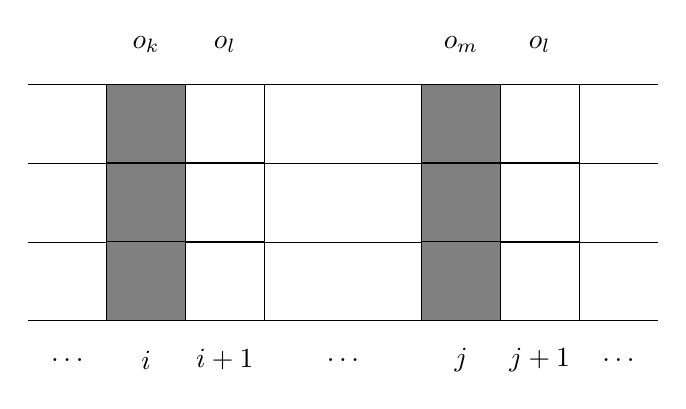
\begin{tikzpicture}
  \tikzstyle{box} = [draw=black, minimum width=10mm, minimum height=10mm];
  \tikzstyle{gray_box}  = [box, fill=gray];
  \tikzstyle{white_box} = [box];


  \draw[very thin] (-1.5, -0.5) -- (6.5, -0.5);
  \draw[very thin] (-1.5, 0.5)  -- (6.5, 0.5);
  \draw[very thin] (-1.5, 1.5)  -- (6.5, 1.5);
  \draw[very thin] (-1.5, 2.5)  -- (6.5, 2.5);

  \node[gray_box]  at (0, 0) {};
  \node[white_box] at (1, 0) {};
  \node[gray_box]  at (4, 0) {};
  \node[white_box] at (5, 0) {};

  \node[gray_box]  at (0, 1) {};
  \node[white_box] at (1, 1) {};
  \node[gray_box]  at (4, 1) {};
  \node[white_box] at (5, 1) {};

  \node[gray_box]  at (0, 2) {};
  \node[white_box] at (1, 2) {};
  \node[gray_box]  at (4, 2) {};
  \node[white_box] at (5, 2) {};

  \node at (0, 3) {$o_k$};
  \node at (1, 3) {$o_l$};
  \node at (4, 3) {$o_m$};
  \node at (5, 3) {$o_l$};

  \node at (-1, -1) { $\dots$};
  \node at (0, -1)  { $i$};
  \node at (1, -1)  { $i+1$};
  \node at (2.5, -1)  { $\dots$};
  \node at (4, -1)  { $j$};
  \node at (5, -1)  { $j+1$};
  \node at (6, -1)  { $\dots$};
\end{tikzpicture}
%%% Local Variables:
%%% mode: latex
%%% TeX-master: "../master"
%%% End:

  \caption{Computing the full forward table from the partial table. Note that
    in figures~\ref{fig:exploiting-repetitions}
    and~\ref{fig:infering-viterbi-path} where the sequence was written from
    right to left, i.e.\ the indices were increasing from right to left. The
    indices in this illustration increase from left to right, since it is
    more natural to reason about. The gray boxes indicate columns filled during
    the when computing the table for the compressed sequence. The white columns
    need to be computed in less than $O(N^2)$ time per column.}
  \label{fig:full-forward-table}
\end{figure}

Unfortunately no solution to this problem has been found. Hence, the posterior
decoding cannot be sped up by exploiting repetitions in the observation
sequence. The running time of computing the posterior decoding is then
$O(M N^3 + TN^2)$ which is asymptotically worse than the original posterior
decoding algorithm that runs in $O(TN^2)$. However, note that the alphabet size
$M$ typically is small, so it is expected that the asymptotic running times of
the two algorithms in practice are comparable.

\section{Indexed Posterior Decoding}

In the last section it was discussed that the posterior decoding for an
observation sequence cannot be computed asymptotically faster using the byte-pair
compression. However, if only a part of the posterior decoding is needed
instead of the entire decoding, a theoretical speedup can be obtained.

For indexed posterior decoding not only an input sequence $Y_{1:T}$ and a model
$\lambda$ is given as input, but also two indexes $i,j \in [1:T]$. Instead of
returning the posterior decoding $V_{1:T}$ only the part of the sequence
from index $i$ to $j$ denoted $V_{i:j}$ is returned.

Recall from section~\ref{sec:using-byte-pair} that the columns of the forward
and backward tables, $\alpha'$ and $\beta'$, of the compressed sequence
$Y_{1:T'}'$ are a subset of columns in the tables, $\alpha$ and $\beta$, of
$Y_{1:T}$. Furthermore, recall that a column is computed using the column
immediately to the left or right of the forward and backward algorithms
respectively as seen in equation~\eqref{eq:8} and~\eqref{eq:9}. Using this, the
columns $i$ to $j$ of the forward and backward tables, $\alpha$ and $\beta$,
corresponding to the \emph{subsequence} $Y_{i:j}$ can be found using existing
columns from the forward and backward tables, $\alpha'$ and $\beta'$.

\begin{figure}
  \centering
  \tikzsetnextfilename{subsequence_posterior}
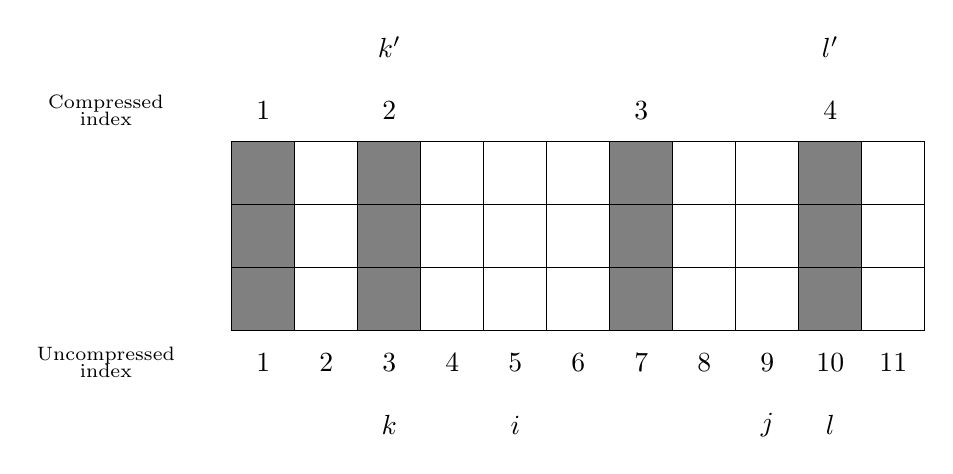
\begin{tikzpicture}
  [scale=0.8]
  \tikzstyle{box} = [draw=black, minimum width=8mm, minimum height=8mm];
  \tikzstyle{gray_box}  = [box, fill=gray];
  \tikzstyle{white_box} = [box];


  \node at (2, 4) {$k'$};
  \node at (9, 4) {$l'$};

  \node[gray_box]  at (0, 0) {};
  \node[gray_box]  at (0, 1) {};
  \node[gray_box]  at (0, 2) {};

  \node[white_box]  at (1, 0) {};
  \node[white_box]  at (1, 1) {};
  \node[white_box]  at (1, 2) {};

  \node[gray_box]  at (2, 0) {};
  \node[gray_box]  at (2, 1) {};
  \node[gray_box]  at (2, 2) {};

  \node[white_box]  at (3, 0) {};
  \node[white_box]  at (3, 1) {};
  \node[white_box]  at (3, 2) {};

  \node[white_box]  at (4, 0) {};
  \node[white_box]  at (4, 1) {};
  \node[white_box]  at (4, 2) {};

  \node[white_box]  at (5, 0) {};
  \node[white_box]  at (5, 1) {};
  \node[white_box]  at (5, 2) {};

  \node[gray_box]  at (6, 0) {};
  \node[gray_box]  at (6, 1) {};
  \node[gray_box]  at (6, 2) {};

  \node[white_box]  at (7, 0) {};
  \node[white_box]  at (7, 1) {};
  \node[white_box]  at (7, 2) {};

  \node[white_box]  at (8, 0) {};
  \node[white_box]  at (8, 1) {};
  \node[white_box]  at (8, 2) {};

  \node[gray_box]  at (9, 0) {};
  \node[gray_box]  at (9, 1) {};
  \node[gray_box]  at (9, 2) {};

  \node[white_box]  at (10, 0) {};
  \node[white_box]  at (10, 1) {};
  \node[white_box]  at (10, 2) {};

  \node[align=center] at (-2.5, 3) {\scriptsize Compressed \\[-2mm] \scriptsize index};

  \node at (0, 3) {1};
  \node at (2, 3) {2};
  \node at (6, 3) {3};
  \node at (9, 3) {4};

  \node[align=center] at (-2.5, -1) {\scriptsize Uncompressed \\[-2mm] \scriptsize index};

  \node at (0, -1) {1};
  \node at (1, -1) {2};
  \node at (2, -1) {3};
  \node at (3, -1) {4};
  \node at (4, -1) {5};
  \node at (5, -1) {6};
  \node at (6, -1) {7};
  \node at (7, -1) {8};
  \node at (8, -1) {9};
  \node at (9, -1) {10};
  \node at (10, -1) {11};

  \node at (4, -2) {$i$};
  \node at (8, -2) {$j$};

  \node at (2, -2) {$k$};
  \node at (9, -2) {$l$};

\end{tikzpicture}
%%% Local Variables:
%%% mode: latex
%%% TeX-master: "../master"
%%% End:

  \caption{Illustration of the computation of the forward (or backward) table
    for a part of the uncompressed sequence given by indices $i$ to $j$,
    given that the columns of the forward table for the compressed sequence,
    shown in gray, have been computed in advance.}
  \label{fig:subsequence-posterior}
\end{figure}

An example of the above is illustrated in
figure~\ref{fig:subsequence-posterior}. Assume that the forward table $\alpha'$
and the backward table $\beta'$ for the compressed sequence has been computed.
This is shown as gray columns. To compute $\alpha$ and $\beta$ from index $i$
to $j$, the computed column at index $k$ with $k \le i$ can be used as a
starting point for the forward computation. In this example that is index 3
that corresponds to the column at index 2 in $\alpha'$. Likewise, column
$l$ with $l \ge j$ can be used as a starting point for the
computation of the backward table.

\subsubsection{Starting Point Columns}

To find the indices $k$ and $l$ for the uncompressed sequence and the
corresponding indices $k'$ and $l'$ for the compressed sequence, a
mapping $M_{uc}$ from uncompressed indices to
compressed indices is created. In this example the map would consist of the
mappings $1 \rightarrow 1, 3 \rightarrow 2, 7 \rightarrow 3$ and
$10 \rightarrow 4$. To find the index $k$ a search is performed on the
map to find the largest key less than or equal to $i$. The value corresponding
to $k$ is $k'$. Likewise, $l$ and $l'$ can be found by finding the smallest key
larger than or equal to $j$.

To compute this mapping, another mapping $M_{sl}$ from each
symbol in the new alphabet $\mathcal{O'}$ to its original length is
created. This can be computed iteratively by inserting first inserting each
original symbol $o_1, \dots, o_M \in \mathcal{O}$ with length 1 into the
map. Next, $o_{M+1}, o_{M+2}, \dots, o_{M'} \in \mathcal{O'}$ is inserted in
the specified order. As each new symbol $o_c \in \mathcal{O'}$ is created using
two existing symbols $o_a$ and $o_b$. The length of $o_c$ can be computed
using the map to obtain the lengths of $o_a$ and $o_b$ and add these two
together.

Now $M_{uc}$ is computed by scanning through the
compressed sequence one symbol at a time while incrementing the corresponding
index in the uncompressed sequence using the map of lengths.

The starting columns for the forward and backward algorithms have now been
found. The only thing missing for the computation is the sequence for which to
compute the following (for forward) or preceding (for backward) columns.

\subsubsection{Sequence}

The simplest solution for finding a sequence for which to compute the forward
and backward tables is to store the original sequence $Y_{1:T}$ and then
extract the sequence $Y_{k:l}$ from that. Instead of storing $Y_{1:T}$,
$Y_{k:l}$ can be found by decompressing $Y_{k':l'}'$ by
replacing the symbols $o_{M + 1}, \dots, o_{M'}$ by symbols from the original
alphabet $\mathcal{O}$. An example of this algorithm is shown in
algorithm~\ref{alg:simple-decompress}. The $\alpha$ and $\beta$ tables can be
found by computing the columns corresponding to $Y_{k:l}$ and afterwards remove
columns $[k, i)$ and $(l, n]$.

\begin{algorithm}
  \caption{Simple decompression algorithm.}
  \label{alg:simple-decompress}
  \begin{algorithmic}[1]
    \Procedure{indexed\_decompression}{$Y', i, j, k, l, k', l'$}
        \State{$Z \gets Y_{k':l'}'$}
        \For{$c = M'$ \textbf{down to} $M + 1$}
          \State{$o_l, o_r \gets $ get\_pair($o_c$)}
          \State{Replace $o_c$ by $o_{l}o_{r}$ in $Z$}
        \EndFor{}
        \State{\Return{$Z$}}
    \EndProcedure{}
  \end{algorithmic}
\end{algorithm}

Decompressing $Y_{k':l'}'$ entirely might be inefficient though. If the
compressed sequence $Y_{1:T'}'$ is highly compressed, i.e.\ $T' \ll T$, the
length of $Y_{k:l}$ might be much larger than $Y_{i:j}$. In the worst case of
$T' = 1$, the decompression would result in the uncompressed sequence
$Y_{1:T}$. Hence, the indexed posterior decoding algorithm will spend a lot of
time computing columns that are thrown away afterwards, and the running time is
$O(M' N^3 + N^2 T)$ which is not an improvement over the original
posterior decoding. The decompression needs to be more clever to improve the
running time.

Observe that only the symbols from index $[i,j]$ need to be from the original
alphabet $\mathcal{O}$. The symbols from $[k, i)$ and $(j, l]$ can be from the
new alphabet, since each column in the these parts of $\alpha$ and $\beta$ are
not needed for the posterior decoding computation. Hence, when decompressing
$Y_{k':l'}'$ symbols that correspond to uncompressed symbols in the interval
$[k, i)$ should not be decompressed, but left as compressed symbols. Likewise,
symbols corresponding to the interval $(j, l]$ should not be decompressed. As
before, symbols corresponding to uncompressed symbols that overlap $[i, j]$
should be decompressed. Is this case the partial decompression of
$Y_{k':l'}'$ resulting in a new sequence $Z$ will then contain symbols
from $\mathcal{O'}$ at the beginning, then symbols from $\mathcal{O}$ in
the middle being the symbols $Y_{i:j}$, and then  symbols from
$\mathcal{O'}$ again in the end.

An algorithm for doing this takes as input a compressed sequence $Y'$ and the
indices $i, j, k, l, k'$ and $l'$. The symbols of subsequence $Y_{k':l'}'$ is
pushed to a stack $Y^S$ such that $Y_{l'}'$ is at the bottom and $Y_{k'}'$ at
the top. The algorithm pops symbols one by one from $Y^S$, while the
corresponding index into the uncompressed sequence $Y$ is maintained using
$M_{sl}$. When a symbol $c$ that overlap $[i, j]$ is encountered $c$ is either
appended to $Z$ if $c \in \mathcal{O}$ or it is split into a pair and pushed to
of $Y^S$ such that the left symbol of that pair will be popped in the next
iteration. The first time a symbol $c \in \mathcal{O}$ overlaps $[i, j]$ is
encountered the index (named \texttt{start\_index}) of that symbol in $Z$ is
saved, as it is used later for computing the posterior decoding. If $c$
overlaps $[k, l]$ it is appended to $Z$. In case there is no overlap between
$c$ and $[k, l]$ nothing is computed, i.e.\ $c$ is thrown away. Pseudo code for
this algorithm is given in algorithm~\ref{alg:decompress}. This algorithm is
much more efficient than algorithm~\ref{alg:simple-decompress} in terms of running
time.

\begin{algorithm}
  \caption{Partially decompress the compressed sequence.}
  \label{alg:decompress}
  \begin{algorithmic}[1]
    \Procedure{indexed\_partial\_decompression}{$Y', i, j, k, l, k', l'$}
        \State{$Z \gets $ nil}
        \State{Stack $Y^S \gets $ nil}
        \State{Push $Y_{l'}', \dots, Y_{k'}'$ to $Y^S$}
        \State{start\_index $\gets$ nil}
        \State{index $\gets k - (M_{sl}(Y^S\text{.top())} - 1)$}
        \While{$Y^S$ is not empty}
            \State{$c \gets Y^S\text{.pop()}$}
            \State{next\_index $\gets$ index + $M_{sl}(c)$]}
            \If{$(\text{index} \le i \land \text{next\_index} > i) \lor
                 (\text{index} > i \land \text{index} \le j)$}
                \If{$c \in \mathcal{O}$} \Comment{$c$ overlaps $[i, j]$}
                    \State{$Z$.append($c$)}
                    \If{start\_index is nil}
                        \State{start\_index $\gets$ $Z$.size() $- 1$}
                    \EndIf{}
                \Else{}
                    \State{$c_l, c_r \gets$ get\_pair($c$)}
                    \State{Push $c_r, c_l$ to $Y^S$}
                    \State{\textbf{continue}} \Comment{Don't update index}
                \EndIf{}
            \ElsIf{$(\text{index} \le k \land \text{next\_index} > k) \lor
                       (\text{index} > k \land \text{index} \le l)$}
                \State{$Z$.append($c$)} \Comment{$c$ overlaps $[k, l]$}
            \EndIf{}
            \State{index $\gets$ next\_index} \Comment{Update index}
        \EndWhile{}
        \State{\Return{$Z$, start\_index}}
    \EndProcedure{}
  \end{algorithmic}
\end{algorithm}

In the previous paragraphs the start columns from $\alpha'$ and $\beta'$, that
is the columns at index $k'$ and $l'$ respectively, have been found. They are
used as the first and last column of the forward table and the backward table for
the partially decompressed sequence $Z$. Furthermore, the sequence $Z$ has
been found. The forward and backward tables of that sequence can now be
computed using the equations~\eqref{eq:8} and~\eqref{eq:9}, but omitting
the base cases as the first (or last) column of the tables has been
computed. As the partially decompressed sequence $Z$ corresponds to the
interval $[k, l]$, but only the posterior decoding for the interval $[i, j]$ is
requested, the posterior decoding should only be computed for that interval.
This is where \texttt{start\_index} is used as it is the index into $Z$
that corresponds to the index $i$ in $Y_{i:j}$. Equation~\eqref{eq:6}
is still used to compute the posterior decoding, but the computation starts at
$t = \mathtt{start\_index}$ and ends at $t = \mathtt{start\_index} + j - i$.

\subsection{Running Time}
\label{sec:running-time-2}

The analysis of the indexed posterior decoding is split into a number of
steps.
\begin{enumerate}
\item Compute $\alpha'$ and $\beta'$;
\item Compute the start columns;
\item Compute the sequence $Z$ corresponding to the columns;
\item Compute the forward and backward tables and the posterior decoding for
  $Z$.
\end{enumerate}
These four steps are now analyzed in turn.

\begin{enumerate}
\item The running time of the forward and backward algorithms is the same as
  for the Viterbi algorithm. If preprocessing/compression of the input string
  $Y_{1:T}$ is not included it takes time $O(M' N^3 + N^2 T')$ to compute
  $\alpha'$ and $\beta'$.

\item Computing the starting point columns requires building the map $M_{sl}$.
  This takes time proportional to the number of symbols, i.e.\ $O(M')$.
  Computing the map $M_{uc}$ requires a scan through the compressed
  sequence. That takes $O(T')$ time.
  Performing the search on the indices of $M_{uc}$ to find the indices
  $k, l, k'$ and $l'$ takes $O(T')$ time. In total this becomes
  $O(M' + T')$.

\item The analysis of algorithm~\ref{alg:decompress} is more complex. In the
  worst case $Y_{1:T'}'$ has length 1, i.e.\ $T' = 1$. The compression of
  $Y_{1:T'}'$ is illustrated as a binary tree seen in
  figure~\ref{fig:decompression}. This is also seen in
  figure~\ref{fig:exploiting-repetitions} where $T' = 5$ and the compression
  corresponds to five binary trees. In this example the compression is
  of the observation sequence $Y_{1:16} = o_1o_1\dots{}o_1$ and corresponds to a
  perfectly balanced tree. Assume that the indexed posterior decoding is
  requested for index $i = 6$ to $j = 14$. Since $T' = 1$, $k' = 1$ and $l'$ =
  1 algorithm~\ref{alg:decompress} will begin at the root of the tree and
  decompress it into two symbols, namely the children of the root. This
  decompression continues for all nodes that are necessary to decompress to
  obtain $Y_{i:j}$. To make the analysis easier to reason about some of the
  nodes in the illustration has been colored. Nodes colored in red or blue correspond to
  symbols that are introduced by decompression of $Y_{1:T'}'$. Nodes without
  coloring correspond to symbols that are not introduced by the decompression. The running time of the
  algorithm is proportional to the number of colored nodes, so to find the
  running time the number of nodes need to be counted.

  The colored nodes are split into two. The blue nodes correspond to symbols
  that are created during the decompression and has descendants that are not
  decompressed. At each level in the tree there are at most two blue nodes.
  Hence, there is at most 2 times the height $h$ of the tree blue nodes. The
  red notes correspond to symbols that are fully decompressed into symbols from
  the original alphabet $\mathcal{O}$. To count the number of these observe
  that the $j - i$ leaves have at most $\frac{j - i + 2}{2}$ parents, at most
  $\frac{j - i + 2}{4}$ grand parents and so on. In this example the leaves and
  their red ancestors correspond to three sub-trees in the tree, but in the
  worst case they correspond to one balanced sub-tree. The size of a balanced
  binary tree with $j - i + 2$ leaves is $2(j - i + 2) - 1$, which is the worst
  case number of red nodes. Summing the number of blue and red nodes we obtain
  $2h + 2(j - i + 2) - 1 = O(h + (j - i))$.

  The height of tree, $h$, can be bounded. The worst case height is obtained
  for sequences that compresses well, that is sequences with many repetitions.
  For unary sequences that the tree has height $h = \log_2 T$ as seen in
  figure~\ref{fig:decompression}. Another class of words that contain many
  repetitions is Fibonacci words. They are generated in a way very similar to
  how Fibonacci numbers are generated by concatenating the two previous words,
  corresponding to generating the next Fibonacci number from the two previous
  ones. Let $S_0$ be ``0'' and $S_1$ be ``01''. Now define
  $S_n=S_{n-1}S_{n-2}$. According to \citet{fraenkel1998many} it is not known
  whether a class of words with more repetitions exist, so for this analysis
  it is assumed that Fibonacci words are worst case. Observe that the number of
  leaves $T$ for a tree of height $h$ is the $h$'th Fibonacci number. In
  general, the $n$'th Fibonacci number can be computed as
  \begin{equation*}
    F_n = \frac{1}{\sqrt{5}}
    {\left(
        \frac{1 + \sqrt{5}}{2}
      \right)}^n
  \end{equation*}
  rounded to the closest integer value. Using this, the height $h$ can be
  bounded in terms of $T$ using that
  \begin{gather*}
      T = \frac{1}{\sqrt{5}} {\left( \frac{1 + \sqrt{5}}{2} \right)}^h \\
      \begin{aligned}
        &\implies
        \begin{aligned}[t]
          \log T & = \log \left( \frac{1}{\sqrt{5}} {\left( \frac{1 + \sqrt{5}}{2} \right)}^h \right) \\
                 & = \log \frac{1}{\sqrt{5}} + \log {\left( \frac{1 + \sqrt{5}}{2} \right)}^h         \\
                 & = \log \frac{1}{\sqrt{5}} + h \log  \frac{1 + \sqrt{5}}{2}                         \\
        \end{aligned} \\
        &\implies h = \frac{\log T - \log \frac{1}{\sqrt{5}}}{\log \frac{1 + \sqrt{5}}{2}} = O\left(\log T\right).
      \end{aligned}
  \end{gather*}
  Hence, the number of colored nodes is no larger than $\log T + (j - i)$,
  which is also the worst case running time of algorithm~\ref{alg:decompress}.

\item Finally the posterior decoding is computed. This takes time proportional
  to the length of the decompressed subsequence. Of course, the subsequence
  contains uncompressed symbols from index $i$ to $j$, but as previously
  discussed the subsequence also contains  symbols corresponding to indices
  $[k, i)$ and $(j, l]$ that may or may not have been decompressed. These are
  drawn as nodes with a thick line in figure~\ref{fig:decompression}. The
  number of these symbols can also be bounded in terms of $T$. Since the
  algorithm does not decompress symbols that corresponds to decompressed
  symbols in the interval $[k, i)$ and $(j, l]$, there is at most be two nodes
  corresponding to these intervals at each layer in the tree. Hence, the number
  of nodes in the intervals is bounded by the height of the tree that is
  $\log T$. The subsequence then has length $j - i + \log T$.

  \begin{figure}
    \centering
    \tikzsetnextfilename{decompression}
\begin{tikzpicture}[
  font=\footnotesize
  ]
  \tikzstyle{level 1}=[level distance=12mm, sibling distance=64mm]
  \tikzstyle{level 2}=[level distance=12mm, sibling distance=32mm]
  \tikzstyle{level 3}=[level distance=12mm, sibling distance=16mm]
  \tikzstyle{level 4}=[level distance=12mm, sibling distance=8mm]
  \tikzstyle{level 5}=[level distance=7mm, sibling distance=8mm]

  \tikzset{
    red/.style = {shape=circle, fill=my-red, draw=black, inner sep=0mm, minimum size=6mm},
    blue/.style = {shape=circle, fill=my-blue, draw=black, inner sep=0mm, minimum size=6mm},
    white/.style = {shape=circle, fill=white, draw=black, inner sep=0mm, minimum size=6mm},
  }

  \node [blue] {$Y_{1:T'}'$}
  child {node [blue]  {}
    child {node [blue, line width=1mm]  {}
      child {node [white] {}
        child {node [white] {$Y_1$} }
        child {node [white] {$Y_2$} }
      }
      child {node [white] {}
        child {node [white] {$Y_3$} }
        child {node [white] {$Y_4$} }
      }
    }
    child {node [red]  {}
      child {node [red] {}
        child {node [red,line width=1mm] {$Y_5$} }
        child {node [red] {$Y_6$}
          child {node {\small $i$} edge from parent[draw=none]}
        }
      }
      child {node [red] {}
        child {node [red] {$Y_7$} }
        child {node [red] {$Y_8$} }
      }
    }
  }
  child {node [blue]  {}
    child {node [red]  {}
      child {node [red] {}
        child {node [red] {$Y_9$} }
        child {node [red] {$Y_{10}$} }
      }
      child {node [red] {}
        child {node [red] {$Y_{11}$} }
        child {node [red] {$Y_{12}$} }
      }
    }
    child {node [blue]  {}
      child {node [red] {}
        child {node [red] {$Y_{13}$} }
        child {node [red] {$Y_{14}$}
          child {node {\small $j$} edge from parent[draw=none]}
        }
      }
      child {node [blue, line width=1mm] {}
        child {node [white]  {$Y_{15}$}}
        child {node [white]  {$Y_{16}$}
        }
      }
    }
  };
\end{tikzpicture}
%%% Local Variables:
%%% mode: latex
%%% TeX-command-extra-options: "-shell-escape"
%%% TeX-master: "../master"
%%% End:

    \caption{The decompression of $Y_{1:T'}'$ using
      algorithm~\ref{alg:decompress} illustrated as a binary tree. In this
      example $Y_{1:T}$ have been compressed to a single character. Hence,
      $T' = 1$}
    \label{fig:decompression}
  \end{figure}

  Computing the forward and backward tables take time
  $O(N^2 (j - i + \log T))$, and computing the posterior decoding using
  equation~\eqref{eq:6} also takes $O(N^2 (j - i + \log T))$ time.
\end{enumerate}
By adding the running times of these four steps a running time of
\begin{gather*}
  O\left(M' N^3 + N^2 T'\right) + O\left(M' + T'\right) + O\left(\log T + (j - i)\right) + O\left(N^2 (j - i + \log T)\right) \\
  = O\left(M' N^3 + N^2 T' + N^2 (j - i + \log T)\right)
\end{gather*}
is obtained for the indexed posterior decoding algorithm.

Note that this is a \emph{worst case} running time. For many practical
applications the compression will not be as good and thus $T' > 1$. In that
case the decompression can be illustrated as $T'$ trees. In many cases only
some of these need to be traversed and the height of them will be
smaller than $\log T$. Furthermore, the $\log T$ term will most likely not
dominate the $j - i$ term. As an example the human genome has length
approximately $3\,000\,000\,000$ base pairs and can be used as the observation sequence
in some bioinformatics applications. As $\log_2 3\,000\,000\,000 \approx 31$ and
$j - i$ probably will be larger, the $\log T$ term does not contribute much
of the running time in most cases.

%%% Local Variables:
%%% mode: latex
%%% TeX-command-extra-options: "-shell-escape"
%%% TeX-master: "master"
%%% End:
